\documentclass[12pt,a4paper,twoside]{book}

\usepackage{hyperref}
\hypersetup{
    colorlinks=true,
    linkcolor=black,
    filecolor=black,      
    urlcolor=green,
    anchorcolor=black,
    citecolor=green
}
\usepackage{amsmath}
\usepackage{graphicx}
\usepackage{subcaption,caption}
\usepackage{subcaption}
\usepackage{tabularx,ragged2e,booktabs}
\usepackage{enumitem}
\usepackage[ruled,longend]{algorithm2e}
\usepackage{booktabs}
\usepackage[numbers,sort&compress]{natbib}
\usepackage{ragged2e}
\usepackage{listings}
\lstset{
 columns=fixed,       
 numbers=left,                         
 numberstyle=\tiny\color{gray},           
 frame=none,                   
 backgroundcolor=\color[RGB]{245,245,244}, 
 keywordstyle=\color[RGB]{40,40,255},         
 numberstyle=\footnotesize\color{black},           
 commentstyle=\it\color[RGB]{0,96,96},          
 stringstyle=\rmfamily\slshape\color[RGB]{128,0,0},
 showstringspaces=false,                      
 language=python,                           
}




%include the configuration file for layout
%Have a look in this file it has some useful commands defined
\usepackage{setspace}
\usepackage{geometry}
\usepackage[toc,page]{appendix}
\usepackage{lipsum}
\usepackage[export]{adjustbox}
\usepackage[T1]{fontenc}
\usepackage{textcomp}
\usepackage{epsfig,graphics}
\usepackage{graphicx}
\usepackage{titlesec}


%%%%%%%%%%%%%%%%%%%%%%%%%%%%%%%%%%%%%%%%%%%%%%%%%%%%%%%%%%%%%%%%%%%%%%%%%%%%%%
% Details of your dissertation
%%%%%%%%%%%%%%%%%%%%%%%%%%%%%%%%%%%%%%%%%%%%%%%%%%%%%%%%%%%%%%%%%%%%%%%%%%%%%%
\newcommand{\projectTitle}{Grammatical Error Correction}
\newcommand{\fullname}{Yucheng Zhang}
\newcommand{\degreeTitle}{<Name of Degree>}
\newcommand{\session}{<Session>}

%%%%%%%%%%%%%%%%%%%%%%%%%%%%%%%%%%%%%%%%%%%%%%%%%%%%%%%%%%%%%%%%%%%%%%%%%%%%%%
% Change the geometry of the page to have a 25 mm binding edge
%%%%%%%%%%%%%%%%%%%%%%%%%%%%%%%%%%%%%%%%%%%%%%%%%%%%%%%%%%%%%%%%%%%%%%%%%%%%%%
 \geometry{
 a4paper,
 total={210mm,297mm},
 left=25mm,
 right=25mm,
 top=25mm,
 bottom=20mm,
 }
 
%%%%%%%%%%%%%%%%%%%%%%%%%%%%%%%%%%%%%%%%%%%%%%%%%%%%%%%%%%%%%%%%%%%%%%%%%%%%%%
% Commands to set the line spacing
%%%%%%%%%%%%%%%%%%%%%%%%%%%%%%%%%%%%%%%%%%%%%%%%%%%%%%%%%%%%%%%%%%%%%%%%%%%%%%
 %\singlespacing
 \onehalfspacing
 %\doublespacing
 
%%%%%%%%%%%%%%%%%%%%%%%%%%%%%%%%%%%%%%%%%%%%%%%%%%%%%%%%%%%%%%%%%%%%%%%%%%%%%%
% Spacing for the chapter header
%%%%%%%%%%%%%%%%%%%%%%%%%%%%%%%%%%%%%%%%%%%%%%%%%%%%%%%%%%%%%%%%%%%%%%%%%%%%%%
 \titleformat{\chapter}[display]
    {\normalfont\Huge\bfseries}{\vspace*{-1\baselineskip}\chaptertitlename\ \thechapter}{15pt}{\huge}
\titlespacing*{\chapter}{0pt}{0pt}{15pt}

\renewcommand\bibname{References}

%%%%%%%%%%%%%%%%%%%%%%%%%%%%%%%%%%%%%%%%%%%%%%%%%%%%%%%%%%%%%%%%%%%%%%%%%%%%%%
% Some shortcuts that maybe useful
%%%%%%%%%%%%%%%%%%%%%%%%%%%%%%%%%%%%%%%%%%%%%%%%%%%%%%%%%%%%%%%%%%%%%%%%%%%%%%
\DeclareTextCommandDefault{\textcopyright}{\textcircled{c}}
 
%%%%%%%%%%%%%%%%%%%%%%%%%%%%%%%%%%%%%%%%%%%%%%%%%%%%%%%%%%%%%%%%%%%%%%%%%%%%%%
% Bibliography style: choose one and make sure you have the relevant .bst file
%%%%%%%%%%%%%%%%%%%%%%%%%%%%%%%%%%%%%%%%%%%%%%%%%%%%%%%%%%%%%%%%%%%%%%%%%%%%%%
\bibliographystyle{abbrv}


%%%%%%%%%%%%%%%%%%%%%%%%%%%%%%%%%%%%%%%%%%%%%%%%%%%%%%%%%%%%%%%%%%%%%%%%%%%%%%
% Layout for the front cover !!!!! YOU SHOULD NOT HAVE TO CHANGE THIS!!!!!
%%%%%%%%%%%%%%%%%%%%%%%%%%%%%%%%%%%%%%%%%%%%%%%%%%%%%%%%%%%%%%%%%%%%%%%%%%%%%%
 
\newcommand{\frontcover}{
% The title page:
\begin{titlepage}
\newgeometry{left=25mm,right=25mm,top=45mm,bottom=0.1cm}

\begin{minipage}[t]{7cm}
\noindent\textbf{\Large{School of Computing}}\\
{\fontfamily{ptm}\selectfont 
\uppercase{faculty of engineering}
}
\end{minipage}
\hfill
\begin{minipage}[t]{7cm}
\vspace*{-25pt}

\includegraphics[scale=0.2,right]{logo_black.png}
\vspace*{-1pt}
\end{minipage}

\noindent\makebox[\linewidth]{\rule{\paperwidth}{0.4pt}}

\centering
\vspace*{37mm}
\textbf{\Large\projectTitle}\\
\vspace*{10mm}
\textbf{\large\fullname}\\
\vspace*{10mm}
\textbf{Submitted in accordance with the requirements for the degree of}\\
\textbf{\degreeTitle}\\
\vspace*{10mm}
\session\\
\restoregeometry
\end{titlepage}
}

%%%%%%%%%%%%%%%%%%%%%%%%%%%%%%%%%%%%%%%%%%%%%%%%%%%%%%%%%%%%%%%%%%%%%%%%%%%%%%
% Define a new environment for the dissertation summary
%%%%%%%%%%%%%%%%%%%%%%%%%%%%%%%%%%%%%%%%%%%%%%%%%%%%%%%%%%%%%%%%%%%%%%%%%%%%%%
\newenvironment{dissertationsummary}
 	{\cleardoublepage \null 
 		\begin{center}%
			\textbf{Summary}
		\end{center}}%
	{\vfill \null }

\begin{document}
%The prelude is everything upto the start of chapter 1


\pagenumbering{roman}
\frontcover

\clearpage
\noindent The candidate confirms that the following have been submitted.\\
<As an example>
\begin{table}[ht!]
\begin{tabular}{|p{0.3\textwidth}|p{0.3\textwidth}|p{0.3\textwidth}|}
\hline 
Items & Format & Recipient(s) and Date \\ 
\hline 
Beliverable 1, 2, 3 & Report & SSO (DD/MM/YY) \\ 
\hline 
Participant consent forms & Signed forms in envelop & SSO (DD/MM/YY) \\ 
\hline 
Deliverable 4 & Software codes or URL & Supervisor, Assessor (DD/MM/YY) \\ 
\hline 
Deliverable 5 & User manuals & Client, Supervisor (DD/MM/YY) \\ 
\hline 
\end{tabular} 
\end{table}

\noindent Type of project: \rule{100mm}{1pt}
\vspace{\fill}\\
\noindent The candidate confirms that the work submitted is their own and the appropriate credit has been given where reference has been made to the work of others.
\vspace{\fill}\\
\noindent I understand that failure to attribute material which is obtained from another source may be considered as plagiarism.
\vspace{\fill}\\
\flushright(Signature of Student) \rule{50mm}{1pt}
\flushleft
\vspace{\fill}
\textcopyright~\session~The University of Leeds and~\fullname
% Summary

\begin{dissertationsummary}
\justifying
This project was about the tradition NLP task “Grammatical Error Correction”, aiming at developing an automatic system which can detect and correct the grammatical errors automatically. The objective is to use TensorFlow to build up and train a sequence to sequence model, that is capable of automatically correcting small grammatical errors in conversational written English, e.g., the messages on mobile phone. Instead of the traditional statistic model and manually rule design, we apply the latest powerful artificial intelligence tools, saying a specific RNN model with LSTM. The details of the configuration of neural network were provided. After building the neural network model, we also train the model on a GPU server and do performance test of it. Besides, we also explain how we overcome the lack of training dataset, i.e., we take English text samples which are known to be mostly grammatically correct and randomly introducing a handful of small grammatical errors to each sentence to produce input-output. As the results revealed, although sometimes the performance was not so good, this neural network model can detect and correct the usual typos which are made in the daily writing sentences. The feasibility of the Seq2seq model under LSTM suggested the promising future of applying artificial intelligence techniques in the grammatical error correction field.
\end{dissertationsummary}

\clearpage
\centering\textbf{Acknowledgements}
\flushleft
\justifying
I would first like to thank my thesis advisor [title] [Name Surname] of the [School / Faculty name] at [University name]. The door to Prof. [Last name] office was always open whenever I get into a trouble or had a question about my research or writing. 

I would also like to thank the experts who were involved in the validation survey for this research project: [List professional Titles, Name and Surnames of the experts who participated/contributed]. Without their passionate participation and input, the validation survey could not have been successfully conducted.

% The contents
\tableofcontents

% The list of figures and tables Uncomments the 3 following lines
%to see a list of tables and list of figures.
%\clearpage
%\listoffigures
%\listoftables

\pagenumbering{arabic}

%include as many chapters as you have.
%the chapters are in a directory called Chapters
\chapter{Introduction}
\label{chapter1}


In language learning, the right usage of vocabularies is very important for non-native speakers when they learn a second language. It is necessary to find out the errors the learners made to help them master a new language. Besides, the automatic grammatical error correction (GEC) system can be needed when people write long documents because people can get bored and ignore many grammatical errors after a long period of work. From these scenarios, we can see that automatic grammatical error correction systems have many potential applications in people’s daily lives. In a word, there is a raising and dramatic request for natural language processing (NLP) techniques which can automatically detect and correct the errors of grammar and word usage which the learners make when they are learning second, or even third languages \cite{leacock2010automated}. To overcome this need, NLP researchers and developers have made a lot of progress in recent years, e.g., the language model, construction of datasets and deep learning techniques, which will be discussed in detail in the literature review.
In recent years, deep learning techniques have shown great power for computer vision and natural language processing \cite{lecun2015deep}. Deep learning techniques are widely used from search engines to recommendation systems in many e-co websites to spam content filtering on social networks with the smartphone playing a more important role in people’s daily life. What’s more, the number of new applications of deep learning is still raising sharply. 

\begin{figure}[ht]
    \centering
    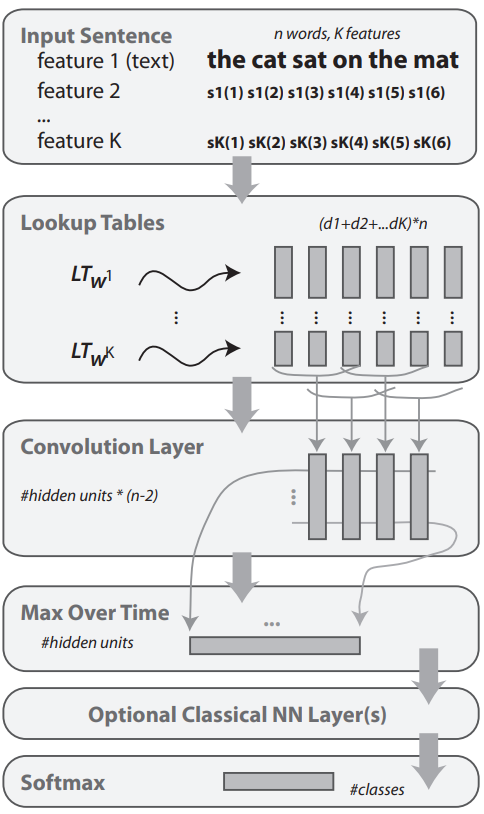
\includegraphics[width=0.5\textwidth]{GDNNNLP.png}
    \caption{A general deep NN architecture for NLP.}
    \label{fig:1}
\end{figure}

In a major part of the research history of NLP, the main methods people apply for NLP problems uses machine learning methods, such as support vector machine (SVM), logistic regression (LR) and shallow neural networks, or even manually designed mechanism with complex rules \cite{young2018recent}. However, these traditional NLP methods run into many problems and can have poor performance. For example, the curse of dimensionality is often met because the representation of language information is often sparse, which leads to a high-dimensional feature expression. What’s more, the traditional NLP methods often depend heavily on manual design, where people often spend a lot of time on writing complex rules. Even though the designers consume so much time on the logical rule design, the mechanism is often incomplete for the fact that the information of human language may change according to different scenarios.

Beside the success of deep learning techniques in computer vision, deep learning also helps to make great progress on NLP with far better performance compared with the traditional NLP methods. A general deep neural network model is shown in Figure~\ref{fig:1}. \cite{collobert2011natural} used a trivial deep learning model to solve NLP problems. The new mechanism at that time outperformed many state-of-art methods, which showed the potential power of deep learning in NLP field. After that time, numerous deep learning NLP methods have been proposed to solve different NLP problem and achieve great success in the different field. The main deep learning applied in NLP includes convolutional neural networks (CNNs), recurrent neural networks (RNNs) and recursive neural networks, which will be explained in detail in later sections.

Applying NLP method to do automatic grammatical error detection and correction is a promising and hot researching area in recent years. A lot of new algorithms and scheme have been proposed to achieve better grammatical error detection and correction. In a word, researchers have done plenty works, which maintain language models, algorithms and dataset. Conll and JFLEG \cite{ng2014conll,napoles2017jfleg} are two famous datasets for the grammatical error correction task. \cite{chollampatt2018multilayer} propose a multilayer convolutional encoder-decoder neural network for grammatical error correction. As the previous neural network model for GEC is time consuming (as it usually takes about several even more than ten days to train a model), \cite{junczys2018approaching} proposal a low resource cost neural networks for GEC task. The works for dataset and neural network model approach will be discussed in detail in the later sections.


\section{Scope}

This project applied the knowledge of deep learning (neural networks), natural language processing, algorithms analysis and basic programming skills. The time spanned from the middle of June to the end of August. The total time period is 11 weeks, of which 2 weeks is spent on literature review, 6 weeks is spent on code implementation and 3 weeks is for the final report. This project is used to detect the grammatical errors made by the beginners of English learning and correct these detected errors into right formats, which has potential applications in many language learning website and mobile applications.

\section{Rationale}
The machine automatic grammatical error correction is a classical researching problem in NLP field. Because of the lack of corpus dataset, the ability of the machine automatic GEC can reach a human-level performance for quite a long time. The new progress on GEC in NLP has been made by applying deep learning techniques. Besides the academic progress, there are many needs in e-co project and smart language teaching. For example, writing is an important part of English learning for non-native speakers and there are large require for detecting and correcting the grammar errors. For the English learners who prepare for English test, e.g., TOFEL or GRE, it would be a large expense if every training passage is commented manually. For the need of grammatical error detection and correction in people’s daily life, this project attempts to build an automatic grammatical error correction system by applying the new techniques of deep learning.

\section{Objective}
The aim of this project is to investigate neural network techniques in NLP for automatic grammatical error correction for writing checking, correction and evaluation applications. First of all, this project constructs a data set which can be used as the training dataset and test dataset for training and testing the deep neural network model in the later steps. Due to the limitation of datasets for grammatical error correction, the famous dataset Conll 2013 and JFLEG are usually perform as test data to evaluate the built GEC system and are difficult to get access. We apply artificial error generation techniques for grammatical error correction proposed by \cite{felice2014generating}. We build a sequence-to-sequence model using long short-term memory (LSTM) encoders and decoders with an attention mechanism as described in \cite{bahdanau2014neural} using stochastic gradient descent. Then, we train the built model based on the previously generated training dataset. Finally, we evaluate the performance of the automatic GEC system using real cases. The focus of this project was on deep learning techniques of NLP on the GEC system which combined grammatical error detection and correction.

\section{Methodology}
\begin{itemize}
    \item Review the context of the application: automatic GEC system for passage evolution. In short, the automatic GEC system should detection the grammatical errors in the test sentence and correct the grammatical errors into the right form. This section will mostly focus on the famous dataset for GEC and well-known works of applying deep learning method for GEC tasks.
    \item 	Review of the pivot of research subject: Seq2seq model with LSTM construction. This neural network model consists of two components, the first of which encodes a source sentence $\mathbf{x}$ and the second $\mathbf{y}$. \cite{sutskever2014sequence} said that RNNs with long short term memory (LSTM) units can achieve close to the state-of-the-art performance of the conventional phrase-based machine translation system. This project will combine the above two models and realize this model by programming.
\end{itemize}
\chapter{Review of Literature}
\label{chapter2}

\section{Grammatical Error Correction}
Grammatical error correction refers to the various tasks to correct the errors in the grammar \cite{ackah2016review}. 
Onwueguzie (2017) simply defined grammatical error correction task as the task to correct the sentence errors. The grammatical errors should be made to be different from other types of errors such as mispellings or mistakes in the omission of the characters in word structure (Onwueguzie, 2017). Grammatical errors are mainly the errors in grammar such as the structure or wrongly usage of subjective words or verbs (Onwueguzie, 2017). Leacock, Chodorow, Gamon and Tetreault (2014) characterize the normal grammatical errors as typographical errors or rule application errors and so on. Therefore, grammatical error correction is defined as the process of correcting any kinds of language usage errors in the grammar domain. 

Grammatical error correction is rather important for various reasons. According to \cite{nassaji2011correcting}, the importance of studying grammatical error correction mainly lies in the aspect that errors in grammar are rather common to see, which is a widespread issue to focus on. In addition, the grammatical errors in scholarly writing domain would generate huge negative influence on the academic writing performance including the message delivery and comprehension standards \cite{nassaji2011correcting}. 
\cite{truscott2007effect} argues that the grammatical error correction is rather effective and crucial to leverage the writers’ capability of writing accurately, which can also help to enhance writing confidence after suitable correction. 
\cite{truscott2007effect} further gets the research conclusion that grammatical error correction will also further enhance the learners’ capability in learning and capturing knowledge by properly arranging the message with better logic. 
It is found that the students being able to write more accurately tend to have better academic and learning performance \cite{fazio2001effect}.

\section{Natural Language Processing}

Natural language processing enjoys a long history and it is crucial to firstly identify its definitions. According to \cite{piotrowski2012natural}, natural language processing refers to the process of using computer systems to process and analyze the data about natural language. Tracing the history of the interactions between computers and language data coding, it can be found that the earliest natural language processing was in the 1950s when there was the article of “Computing Machinery and Intelligence” by Alan Turing (1950), making the formal starting point of the natural language processing. However, even before 1950, there were numerous scholars proposing the concepts of “language as a science” “the language relationship is the source of meaning creation” and “the shared norms to influence the decisions made by individuals” 
\cite{piotrowski2012natural}. These concepts paved the road that language could be structured and processed by turning the language systems into a digital system 
\cite{piotrowski2012natural}. Later since the 1980s, with the development of technology and evolution of society, natural language processing is then coming into use with the development of artificial intelligence \cite{kumar2011natural}. Artificial intelligence is the basic technology enabling the computers to comprehend and take advantage of the languages of human beings, which makes a possible for computers to have a dialogue with people \cite{bhirud2017grammar,kumar2011natural}. The great popularity of this technology was in 1990s while in the 21st century, the new NLP system was developed continuously, making the great progresses of the world \cite{kumar2011natural}.

\section{GEC Dataset}
Grammatical Error Correction has various datasets such as Conll and JFLEG \cite{ng2014conll,napoles2017jfleg}. The CoNLL-2013 dataset was defined to share the message of grammatical errors, so various task takers can share the correction works with evaluations of peers’ works. The primary goal of the CoNell dataset is to evaluate algorithms and systems in an automatic way enabling the function of correcting grammars for second-language English learners \cite{ng2014conll}. For JFLEG (full name of Fluency-Extended GUG Corpous), it is developed to evaluate the correction performance of various grammatical mistakes with 747 English sentences with 4 references separately \cite{napoles2017jfleg}. Two main goals for the grammatical performance checking based on this system are fluency and grammaticality \cite{napoles2017jfleg}. It is argued that the distinctiveness of JFLEG dataset is that it helps to present a comparable broader range of “language proficiency levels and uses holistic fluency edits” in the process of correcting the errors in grammar settings, which is also helpful to turn the original writing be more fluent and native \cite{napoles2017jfleg}. Therefore, from these two scholars’ opinions, it can be found that CoNll and JELEG dataset are both designed to test and correct the errors in grammar, but they share with each other the differences from aspects of core goals and functions.

\section{GEC Research}
There are also scholarly articles focusing on the work of grammatical error correction. \cite{bhirud2017grammar} argue that to better manage the process of grammatical error correction, it would be important to firstly characterize the common grammatical errors. There are 8 big categories of grammatical errors listed by \cite{bhirud2017grammar} named punctuational errors, constituents’ agreements errors, modifier being misplaced, pronominal reference being valuely presented, incorrect choice of words and no appropriate vocabulary, a shortage of the parallel structure, the sprawl issues in the sentences, and the problems lying in tense and modality agreements. However, \cite{soni2018systematic} categorize the grammar errors into several dimensions named frequency error, validity of text, standards of one error, the nature of one error, and error type overlapping problems. In the grammatical error checking process, it would be rather important to consider the role played by the grammatical error checker which constitutes both human quality checkers and artificial intelligence technology-based checkers \cite{bhirud2017grammar}. Grammar checking is the fundamental task to check where and what the problems are, and the severity of the errors \cite{bhirud2017grammar}. For a grammar quality checker, the normal working routines follow the following steps in the work: 
\begin{itemize}
    \item to segment and tokenize the sentences through cutting a whole sentence into several parts into the units of morphemes.
    \item to do the morphological analysis.
    \item to do the POS tagging job named part-of-speech tagging.
    \item and to parsing stage issues by checking the syntactic constraints in the overall hierarchical structure \cite{bhirud2017grammar}.
\end{itemize}

\cite{bhirud2017grammar} also develop three approaches for grammar checking named rule-based checker, data driven grammar checker and hybrid grammar checker. For rule-based checking mechanism, according to \cite{naber2003rule}, it needs the grammar checker to firstly characterize the features of grammar rules, develop the rules and then testing the rules, based on which it would compare the rules patterns within the existing sentence structure with the newly set language rules. It is argued that rule-based grammar checking began in the 1980s which focused on the area of language learning, and later, the rule-based grammar checking was applied in technological domain with the help of Microsoft Word to help to detect the grammar mistakes \cite{nazar2012google}. Rule-based grammar checking process has its advantages by overcoming the various barriers or obstacles through knowledge approaches or statistical approaches \cite{nazar2012google}. 

As for the data driven grammar checker, according to \cite{naber2003rule}, it refers to the process of checking grammar errors through drawing the data based on the journals, magazines and other online resources to get the corpus. \cite{naber2003rule} also points that the data-driven grammar checking approach has two sub methods named corpus based one and the one trying to check the input contents of texts through probabilistic methods. Data-driven grammar checking have two systems named MST and Malt system \cite{plank2010grammar}. For MST Parser, it is a graph-oriented dependency parser while the Malt system was a transition-based dependency parser, according to \cite{plank2010grammar}. The third one is hybrid method for grammar checking which refers to the process of utilizing the two approaches of data-driven approach and rule-based approach together at one time to check and correct the errors in one text \cite{bhirud2017grammar}. According to \cite{bhirud2017grammar}, the hybrid approach is more complex to use, asking for higher capabilities of quality checkers, but the overall grammar quality checking result can be better. 
Besides these three approaches of grammar error checking, it is argued by \cite{soni2018systematic} that with the development of technology, the grammar checking tools have also experienced the various stages from the writer’s workbench in the 1980s to the commercialized software package in the 1990s. In the 21st century with the fast development of web 2.0 and the associated information technology, there are a variety of the grammar checking techniques and tools such as Language Tool and other automatic grammar error detection systems on computers \cite{soni2018systematic}.

From these scholars’ ideas, it can be learned that the works of grammatical error checking have been experienced a huge development speed by capturing the trend of technology, web 2.0 and the application of specific approaches. Grammatical error checking is thus not only a process in theoretical domain but also the technical domain. However, the GEC approaches described above have their own drawbacks though they achieved state of the art at that time. The short comings are summarized below.
\begin{itemize}
    \item Rule-based approaches have poor generalization ability. It requires extensive effort to build the rule set. Regardless of the size of the rule set, considering the variability of the human languages, it seems impossible to cover all possible errors and there are lots of exception to the rules.
    \item Data driven approaches consume too much resources, e.g., memory. They also require large and domain adapted datasets to avoid the data-scarceness specific issues. In addition, they usually lack semantic information and favoring high-occurring events is not always the best way of detecting and correcting grammatical errors.
    \item Hybrid approaches maintain some drawbacks of rule-based approaches and data driven approaches since they ensemble both types. They may require many resources for statistical part as well as much time for rule design.
\end{itemize}
\section{Main Techniques}
The literature also identifies two main techniques for grammar error checking named Seq2seq Model and Long Short-term Memory Model \cite{lu2019advances}. 
We use Seq2seq model with LSTM based on the following reasons.
\begin{itemize}
    \item Seq2seq models with LSTM can generate arbitrary output sequences after seeing the entire input. They can even focus in on specific parts of the input automatically to help generate a useful translation.
    \item Seq2seq models have achieve great success in GEC area. Recent Seq2seq based GEC systems \cite{chollampatt2018multilayer,ge2018fluency,ge2018reaching}  can achieve human-level performance in GEC benchmarks.
\end{itemize}

\subsection{Seq2seq Model}
For Seq2seq model, according to \cite{lu2019advances}, it is used by selecting a foundational dataset which is given already, and then take the inputs situations into consideration to predict the outputs. The following Figure~\ref{fig:2} illustrates the example of the Seq2seq Model which incorporates both inputs situation and outputs situation \cite{lu2019advances}. The ABC are the input sequences while the WXY are the output sequences. Seq2seq model is also called encoder-decoder model and the purpose of the model is to translate some language texts from one to another based on some systematic processing systems \cite{schmaltz2016sentence}. It has the advantage of enabling the grammar checker to check the sentence-level errors and issues to a thorough way \cite{schmaltz2016sentence}. 
Other scholars \cite{szuba2001computational} state that Seq2Seq model is a rather useful framework for machine learning and machine translation which contains these steps named text summary, modeling of the conversations, capturing the images and so on. It is argued that Seq2Seq model is an encoder-decoder mechanism, so with the inputs to a system, it would also characterize the outputs \cite{szuba2001computational}. Therefore, it can be learned that the Seq2Seq model is a type of model enhancing the artificial intelligence technological performance \cite{szuba2001computational}. It also means that the model is helpful to characterize the comprehension of the natural languages in the process characterizing the grammar errors. 
\begin{figure}[ht]
    \centering
    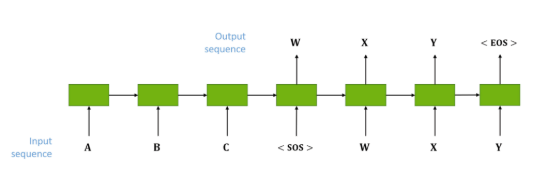
\includegraphics[width=\textwidth]{Seq2seqAE.png}
    \caption{Seq2Seq Architecture Example.}
    \label{fig:2}
\end{figure}

\subsection{Long Short-Term Memory}

The long short-term memory is an important neural network to better characterize the meanings in the area of deep learning \cite{hochreiter1997long}. Long short-term memory mechanism is widely applied in the studies of recognition of the handwriting. As shown in the following Figure 2, it can be found that the system is composed by inputs and outputs \cite{hochreiter1997long}. According to \cite{hochreiter1997long}, a comprehensive long short-term memory system is usually composed by various parts named cell, input gates, output gates and forget gate. The long short-term memory model has been applied in many situations including the memory training process and improving the learning effects. Applying the model in grammar error correction, the long short-term memory is thought to be rather crucial to leverage the overall quality standards when people are trying to memorize the grammar rules and seek further improvements \cite{zheng2016chinese}. Scholars of \cite{hochreiter1997long} point that long short-term memory is a kind of artificial recurrent neural network architecture, which is a key component to help to enhance deep learning. It is said by \cite{hochreiter1997long} that long short-term memory mechanism has its uniqueness by enhancing the feedback providing, so it can ensure the long-term entire sequence of data collection. It is thus an important perspective of grammar error collection. 


\begin{figure}[ht]
    \centering
    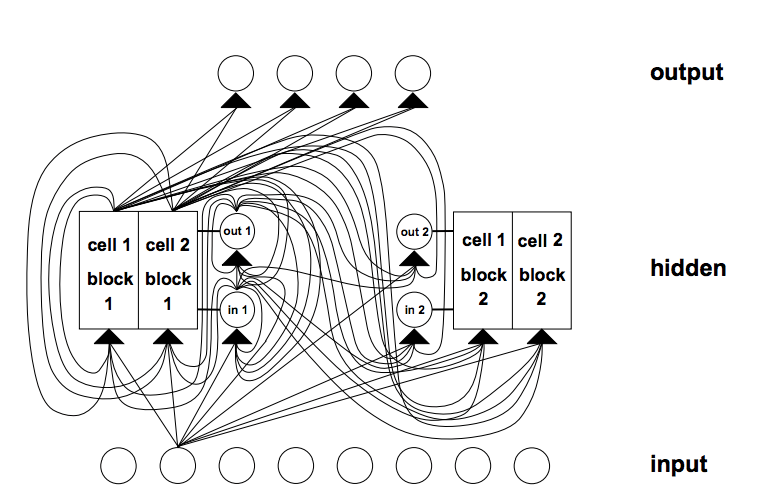
\includegraphics[width=\textwidth]{LSTM.png}
    \caption{Long Short-term Memory Model.}
    \label{fig:3}
\end{figure}
\chapter{Key Structures}
\label{chapter3}

In this project, we build a sequence-to-sequence (seq2seq) model using LSTM encoders and decoders with which is similar to the seq2seq model described in \cite{bahdanau2014neural}. The seq2seq model is also known as encoder-decoder model, which are widely used in machine translation from a source language to a target language. Thus, the encoder-decoder model can also be used for GEC task, where the encoder network can be used for encoding the potentially error source sentences in the vector space and the decoder network can be used for generating the corrected output sentences by using the source encoding, saying that we treat the error  sentences as the source language and treat the corresponding correct sentence as another language (the target language).

\section{Problem Formulation}
In the part, we will apply the theoretic tool to formulate the GEC problem, which can become a good base for the later analysis and problem solution description. By using the tools of the probabilistic theory and optimization theory, the GEC task problem can be formulated as the following problem, where the designers are requested to find a correct sentence $\mathbf{y}$ that maximizes the conditional probability of the case where the correct sentence is $\mathbf{y}$ given a source sentence $\mathbf{x}$, i.e.,

$${\rm argmax}_\mathbf{y}p\left(\mathbf{y}| \mathbf{x}\right).$$

In order to get a proper neural network model, we need to train a parameterized model which can maximize the conditional probability of the case where the correct sentence is $\mathbf{y}$ given a source sentence $\mathbf{x}$, using a parallel training corpus (source input words and target input words as shown in Figure~\ref{fig:4}). Once the conditional distribution is learned by the model (a translation model), given a source sentence a corresponding correction can be generated by searching for the sentence that maximizes the conditional probability.

\begin{figure}[ht]
    \centering
    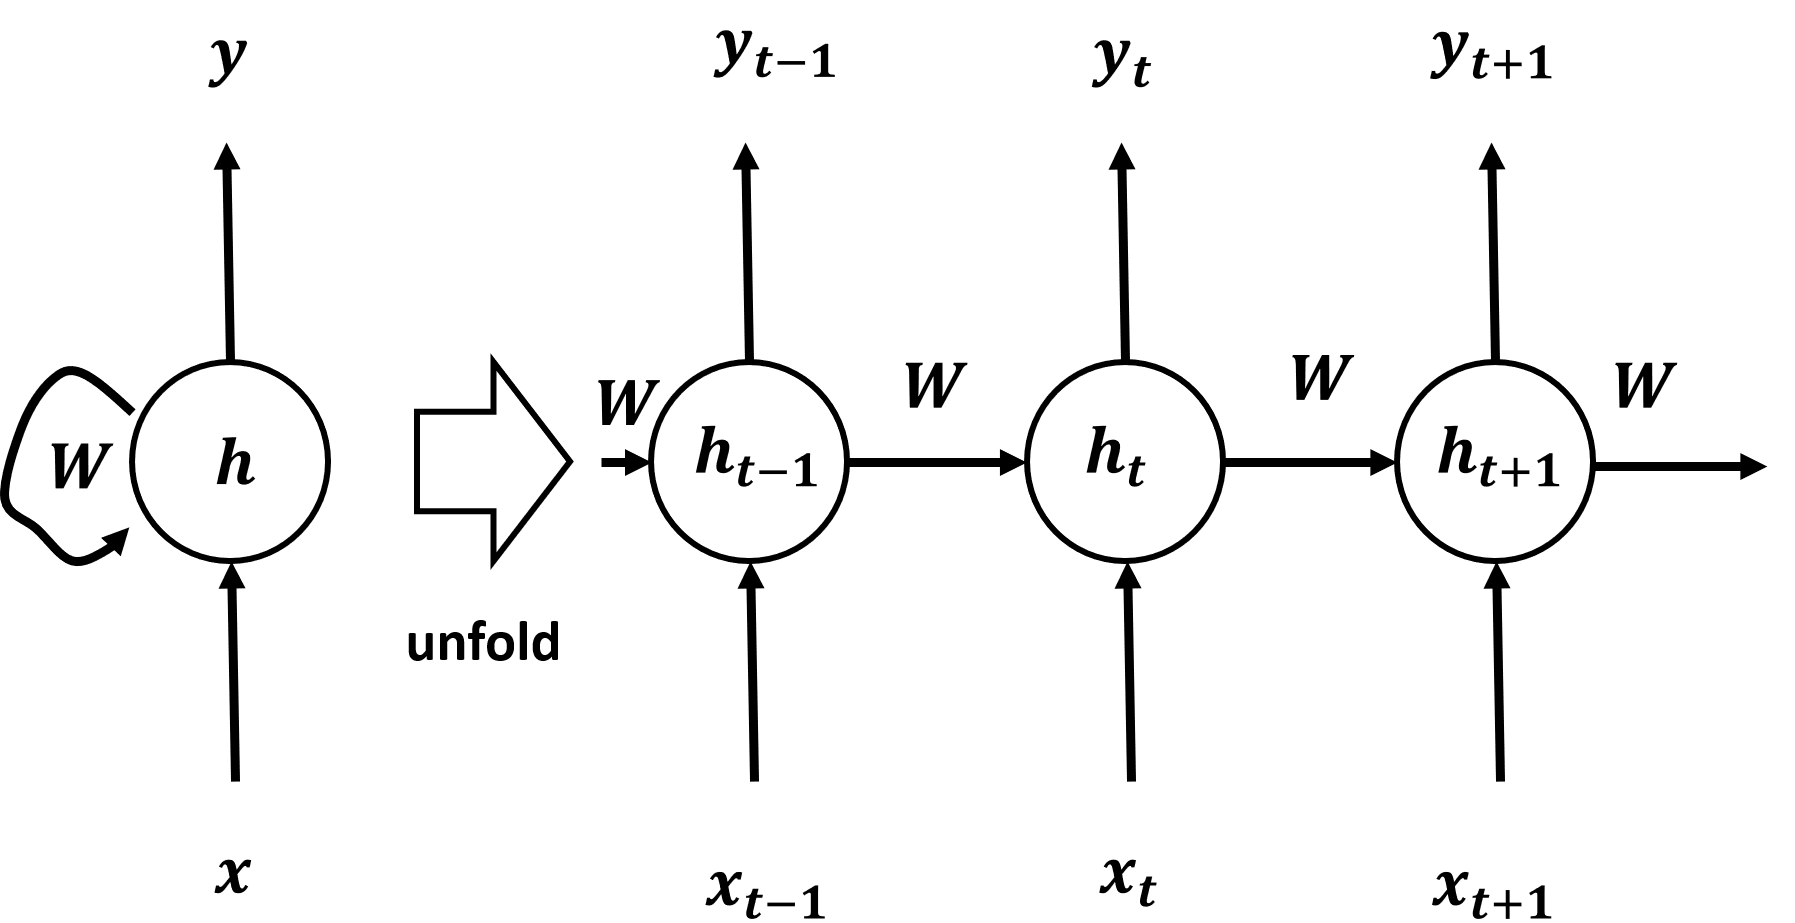
\includegraphics[width=\textwidth]{RNN.png}
    \caption{A recurrent neural network and the unfolding in time of the computation involved in its forward computation.}
    \label{fig:4}
\end{figure}

\section{RNN Encoder–Decoder}

In this part, we will describe briefly the underlying framework, called RNN Encoder–Decoder, which is originally proposed by \cite{cho2014learning,sutskever2014sequence}. The novel architecture we build is also based on the above RNN Encoder–Decoder. Thus, it is necessary to have a detailed description about the RNN Encoder-Decoder model. In this model, there are two RNN, one of which is responsible for encoding the input sequence into a fixed length vector representation and another of which is responsible for decoding that representations into another sequence of symbols. Usually, they are jointly trained to maximize the conditional probability of the target sequence $\mathbf{y}$ given the input sequence $\mathbf{x}$ and the standard log loss of recurrent neural network is used to improve empirical performance. This part will provide a detailed description on RNN and seq2seq model which will be used in our built model.

\subsection{Preliminary: Recurrent Neural Networks}
The insights behind RNNs is to make full utilization of the sequential information of the input data. For a traditional neural network, we know before, we usually make an assumption that all input samples (or even the output data) should be independent of each other. But in many real tasks, that assumption is not a good idea. For example, if you want to predict the next word in a sentence, you had better to know the words that come before it. In this example, the input words are dependent on the words before them, which is beyond the assumption of the traditional neural networks. For this requirement, RNNs are proposed. RNNs are called recurrent for the fact that they do the same task for every element of a sequence and output a result which is dependent on the previous computations. In other word, we can think about RNNs that they have a “memory” which store the information about what has been calculated so far. From theoretic aspects, RNNs can make use of information in arbitrarily-length sequences. However, in practice, RNNS are limited to looking back just only a few steps. The following will give a theoretical formulation of the RNNs which is shown in Figure~\ref{fig:4}.

According to \cite{cho2014learning}, the recurrent neural network (RNN) is a special kind of neural network, which consists of a hidden state $\mathbf{h}$ and an optional output $\mathbf{y}$ which operates on a variable-length sequence $x=\left(x_1,\ldots,x_T\right)$. At each time step t, the hidden state $\mathbf{h}_{<t>}$ of the RNN is updated by 
$$\mathbf{h}_{<t>}=f\left(\mathbf{h}_{<t-1>},x_t\right),$$
where $f$ is a non-linear activation function. $f$ can be any kind of functions, saying that $f$ may be as simple as an element-wise logistic sigmoid function or even as complex as a long short-term memory (LSTM) unit. An RNN can be trained to learn the probability distribution over a sequence to predict the next symbol in the sequence. In that case, at each timestep $t$, the output is the conditional distribution $p\left(x_t| x_{t-1},\ldots,x_1\right)$, where $(x_{t-1},\ldots,x_1)$ is the previous sequence and $x_t$ is the current symbol we need to predict. For example, we can consider a multi-nomial distribution (1-of-K coding) can be output by using a softmax activation function. The probability of the value of each current element can be expressed as the following
$$p\left(x_{t,j}=1| x_{t-1},\ldots,x_1\right)=\frac{\exp(\mathbf{w}_j\mathbf{h}<t>)}{\sum_{j'=1}^{K}\exp(\mathbf{w}_{j'}\mathbf{h}<t>)},$$
for all possible symbol $j=1,\ldots,K$, where $\mathbf{w}_j$ are the rows of a weight matrix $\mathbf{W}$. By combining these probabilities, we can compute the probability of the sequence $\mathbf{x}$ using
$$p\left(x\right)=\prod_{t=1}^{T}{p\left(x_t=1 | x_{t-1},\ldots,x_1\right)}.$$
From this learned distribution, it is straightforward to sample a new sequence by iteratively sampling a symbol at each time step.

\subsection{Seq2seq Model}

Seq2seq model is a type of RNNs, which has been applied in many area now, such as machine translation, speech recognition, video captioning, etc. This model was first introduced by google in their machine translation system \cite{sutskever2014sequence}, which was shown to outperform all the existing state of arts at that time. Before that, the translation worked in a very naive way which is that each word that users use to type was converted to its target language giving no regard to its grammar and sentence structure. From this aspect, the seq2seq model revolutionized the process of translation by making use of deep learning. Because It not only considers the current word/input while translating but also its neighboring word in the sentences, which is really a big step.

In the Seq2seq framework, an encoder reads the input sentence, a sequence of vectors $x=\left(x_1,\ldots,x_T\right)$, into vector c. Although most of the previous works use to encode a variable-length input sentence into a fixed-length vector, e.g., \cite{cho2014learning}, it is not necessary actually. The most common approach is to use an RNN such that
$$\mathbf{h}_{<t>}=f\left(\mathbf{h}_{<t-1>},x_t\right)$$
and
$$c=q\left(\left\{h_1,\ldots,h_T\right\}\right),$$
where $h_t\in\mathbf{R}^n$  is a hidden state at time $t$, and $c$ is a vector generated from the sequence of the hidden states. $f$ and $q$ are some nonlinear functions. We use LSTM as $f$ and 
$$q\left(\left\{h_1,\ldots,h_T\right\}\right)=h_t.$$
The decoder is often trained to predict the next word $y_{t’}$ given the context vector $c$ and all the previously predicted words 
$$y_1,\ldots,y_{t’}.$$
In other words, the decoder defines a probability over the correction $\mathbf{y}$ by decomposing the joint probability into the ordered conditionals:
$$p\left(\mathbf{y}\right)=\prod_{t=1}^{T}{p\left(y_t|\left\{y_{t-1},\ldots,y_1\right\},c\right)},$$
where 
$$\mathbf{y}=(y_1,\ldots,y_T).$$
With an RNN, each conditional probability is modeled as
$$p\left(y_t|\left\{y_{t-1},\ldots,y_1\right\},c\right)=g\left(y_{t-1},s_t,c\right),$$
where $g$ is a nonlinear, potentially multi-layered, function that outputs the probability of $y_t$, and $s_t$ is the hidden state of the RNN.
Usually, the two components, i.e., encoder and decoders, of the seq2seq model are jointly trained to maximize the conditional log-likelihood
$$\max_\mathbf{\theta}{\frac{1}{N}\sum_{n=1}^{N}{\log{p_\mathbf{\theta}}\left(\mathbf{y}_n\middle|\mathbf{x}_n\right)}}$$
where $\mathbf{\theta}$ is the model parameter set and the $(\mathbf{x}_n,\mathbf{y}_n)$ is the (input sequence, output sequence) pair from the training set.

\begin{figure}[ht]
    \centering
    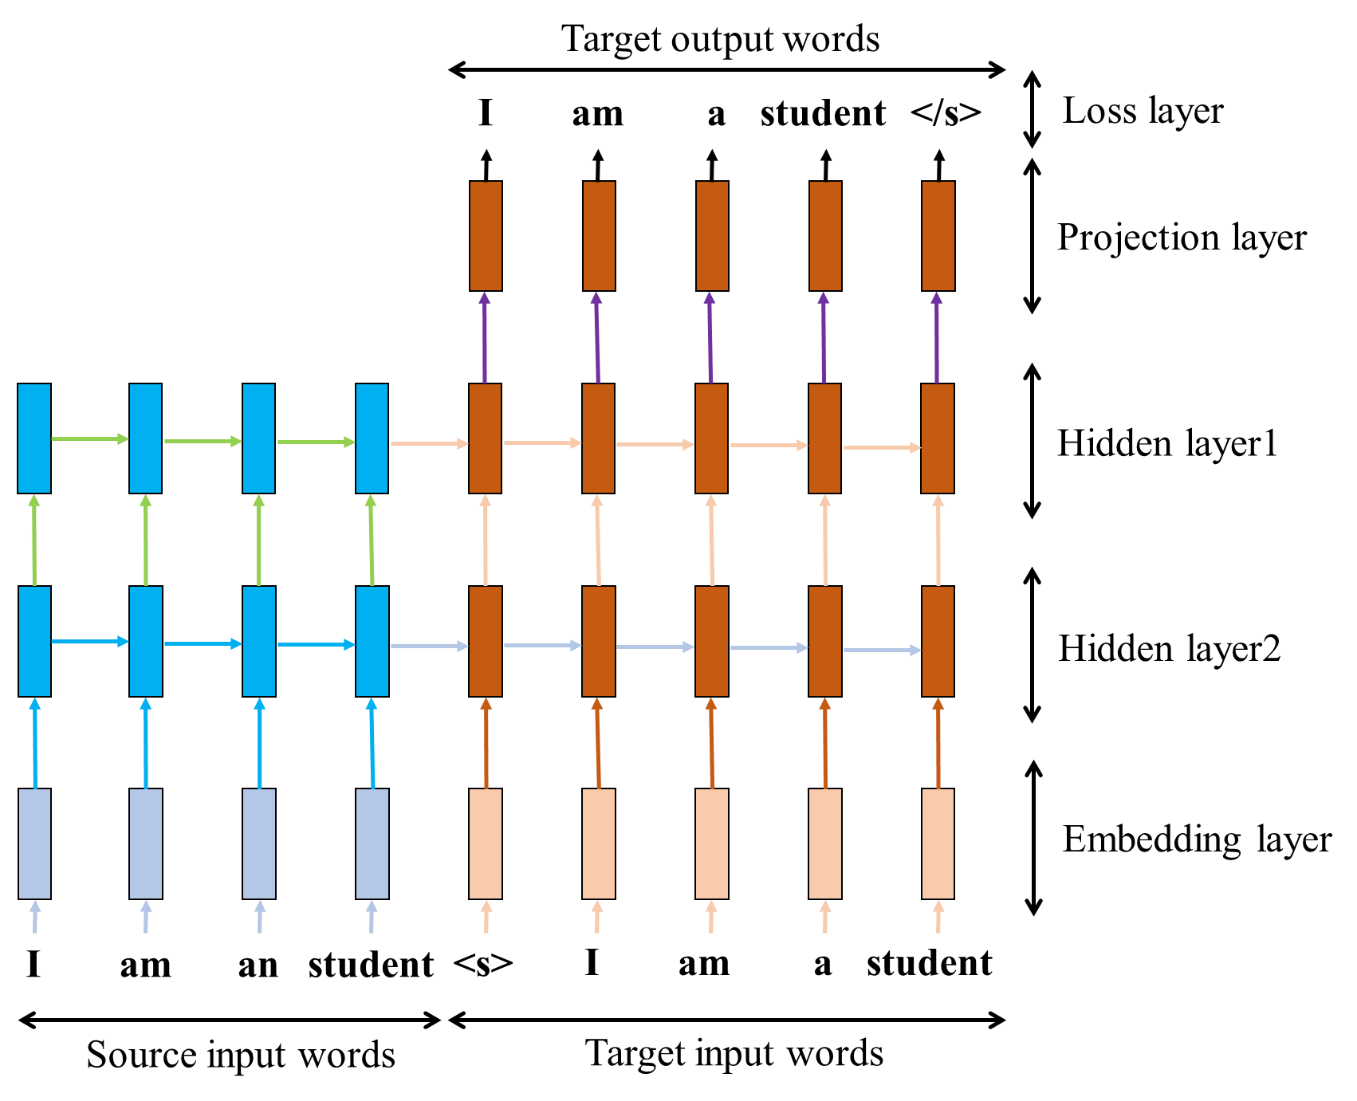
\includegraphics[width=\textwidth]{NMC.png}
    \caption{Neural Machine Correction – example of a deep recurrent architecture proposed by for correct a source sentence "I am an student" into a target sentence " I am a student ". Here, "<s>" marks the start of the decoding process while "</s>" tells the decode.}
    \label{fig:4}
\end{figure}


\chapter{Architecture}
\label{chapter4}


In the section, we will provide detailed description of the architecture of neural networks for automatic GEC task. The architecture consists of a bidirectional RNN as an encoder and a decoder that emulates searching through a source sentence during decoding a correction. The architecture of the neural network model we built is shown in the following figure.

\begin{figure}[ht]
    \centering
    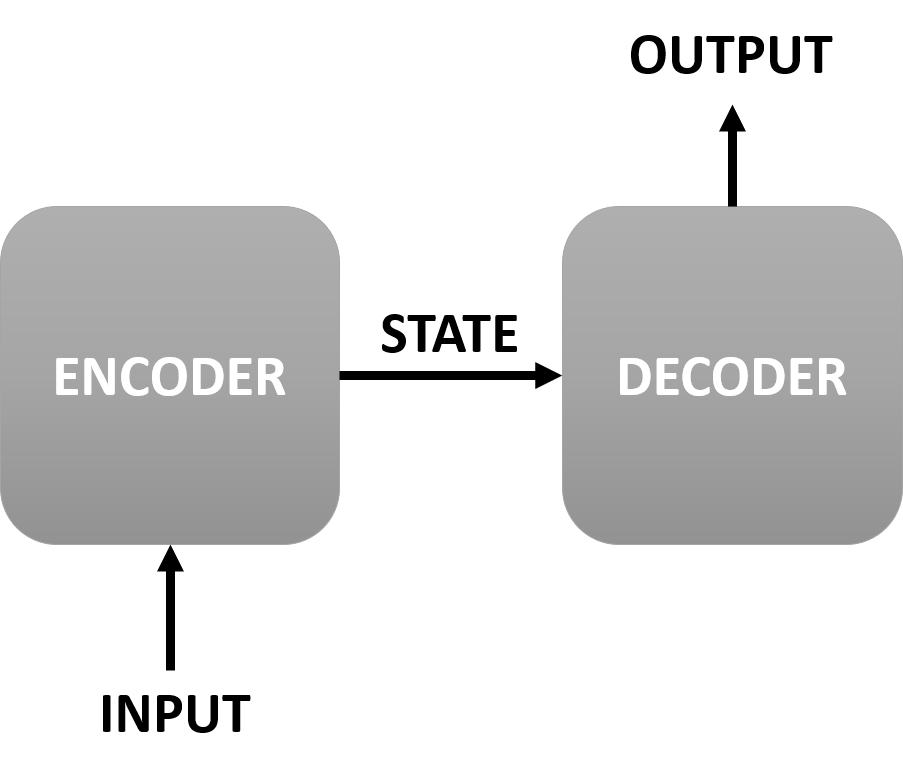
\includegraphics[width=0.8\textwidth]{EDA.png}
    \caption{Encoder and Decoder Structure.}
    \label{fig:5}
\end{figure}

\section{Decoder}

As the illustration in Section 3, the encoder is to read the input sentence, a sequence of vectors $\mathbf{x}=\left(x_1,\ldots,x_T\right)$, and convert the input sentence into a vector $c$. As the encoder reads each symbol, the hidden state of the RNN for each step, saying $h$, changes as the equations shown in the last section.

In this model architecture, we define each conditional probability as:
$$p\left(y_i\middle|\left\{y_{i-1},\ldots,y_1\right\},\mathbf{x}\right)=g\left(y_{i-1},s_i,c_i\right),$$
where $s_i$ is an RNN hidden state for time $i$, computed by
$$s_i=f\left(s_{i-1},y_{i-1},c_i\right).$$
Please note that the approach here is different from the traditional encoder–decoder approach. Here, the probability is conditioned on a distinct context vector $c_i$ for each target word $y_i$ while the traditional one is conditioned on the sequence.

The context vector $c_i$ depends on a sequence of annotation $\left\{h_1,\ldots,h_T\right\}$ to which an encoder maps the input sentence. Each annotation $h_i$ contains information about the whole input sequence with a strong focus on the parts surrounding the $i$-th word of the input sequence.

The context vector $c_i$ is, then, computed as a weighted sum of these annotations $h_i$:
$$c_i=\sum_{j=1}^{T}\alpha_{ij}h_j.$$
The weight $\alpha_{ij}$ of each annotation $h_j$ is computed by
$$\alpha_{ij}=\frac{\exp\left(e_{ij}\right)}{\sum_{k=1}^{T}\exp\left(e_{ik}\right)},$$
where 
$$e_{ij}=a\left(s_{i-1},h_j\right).$$
is an alignment model which scores how well the inputs around position $j$ and the output at position $i$ match. The score is based on the RNN hidden state $s_{i-1}$  and $j$-th annotation $h_j$ of the input sentence.

We parametrize the alignment model as a feedforward neural network which is jointly trained with all the other components of the proposed system. Note that unlike in traditional machine translation, the alignment is not considered to be a latent variable. Instead, the alignment model directly computes a soft alignment, which allows the gradient of the cost function to be backpropagated through. This gradient can be used to train the alignment model as well as the whole translation model jointly. 

We can understand the approach of taking a weighted sum of all the annotations as computing an expected annotation, where the expectation is over possible alignments. Let $\alpha_{ij}$ be a probability that the target word $y_i$ is aligned to, or corrected from, a source word $x_j$. Then, the $i$-th context vector $c_i$ is the expected annotation over all the annotations with probabilities $\alpha_{ij}$.

The probability $\alpha_{ij} $, or its associated energy $e_{ij}$, reflects the importance of the annotation $h_j$ with respect to the previous hidden state $s_{i-1}$ in deciding the next state $s_i$ and generating $y_i$. Intuitively, this implements a mechanism of attention in the decoder. The decoder decides parts of the source sentence to pay attention to. By letting the decoder have an attention mechanism, we relieve the encoder from the burden of having to encode all information in the source sentence into a fixed length vector. With this new approach the information can be spread throughout the sequence of annotations, which can be selectively retrieved by the decoder accordingly.

\begin{figure}[ht]
    \centering
    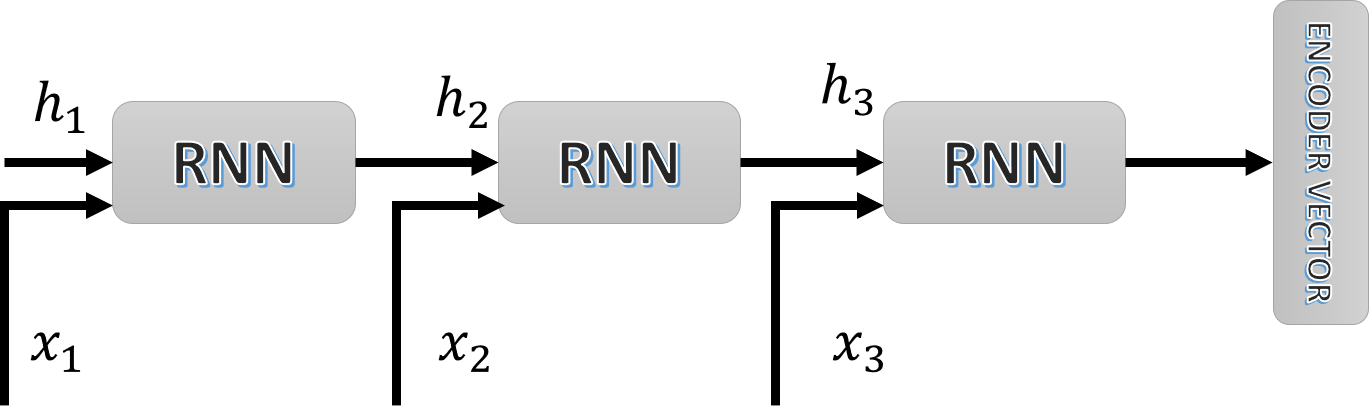
\includegraphics[width=0.8\textwidth]{ECODER.png}
    \caption{Structure of Encoder.}
    \label{fig:6}
\end{figure}

\section{Encoder}
The usual RNN reads an input sequence $\mathbf{x}$ in order starting from the first symbol $x_1$ to the last one $x_T$ . However, in the proposed scheme, we would like the annotation of each word to summarize not only the preceding words, but also the following words. Hence, we use a bidirectional RNN \cite{schuster1997bidirectional}.

A BiRNN consists of forward and backward RNN’s. The forward RNN $\vec{f}$ reads the input sequence  as it is ordered and calculates a sequence of forward hidden states $\left({\vec{h}}_1,\ldots,{\vec{h}}_T\right)$. 
The backward RNN $f$ reads the sequence in the reverse order (from $x_T$ to $x_1$), resulting in a sequence of backward hidden states $\vec{h}_1,\ldots,{\vec{h}}_T$. 
We obtain an annotation for each word $x_j$ by concatenating the forward hidden state ${\vec{h}}_j$ and the backward one ${\bar{h}}_j$ , i.e., $h_j=[\vec{h}_j^T;\bar{h}_T^T]T$. 
In this way, the annotation $h_j$ contains the summaries of both the preceding words and the following words. Due to the tendency of RNNs to better represent recent inputs, the annotation $h_j$ will be focused on the words around $x_j$ . This sequence of annotations is used by the decoder and the alignment model later to compute the context vector.

\begin{figure}[ht]
    \centering
    \includegraphics[width=0.8\textwidth]{Decoder.png}
    \caption{Structure of Decoder.}
    \label{fig:7}
\end{figure}
\chapter{Implementation}
\label{chapter5}


In section, we will explain the implement of the seq2seq model with LSTM, which has been described in Section~\ref{chapter3} and Section~\ref{chapter4} in detail. Besides the implementation, the method of processing and generating the training and testing dataset will also be introduced in this section. Then, we will train a neural network model by using the generated training dataset and evaluate the trained network model by the generated testing dataset. In a word, we will describe the dataset, implementation, training and evaluation in the following.

\section{Dataset}
Building error correction systems by applying the machine learning techniques usually needs a large amount of annotated data, which is difficult to obtain. In addition, the available error-annotated corpora are often focused on specific groups of people (e.g. non-native students), error types (e.g. spelling, syntax), genres (e.g. university essays, letters) or topics. Consequently, we cannot grantee that these datasets is representative enough for training the models and or the trained GEC system is general enough in different scenarios. On the other hand, building new corpora is not always a viable solution since error annotation by human is expensive. Focusing on the existing dataset, the grammatical error correction has various datasets such as Conll and JFLEG \cite{ng2014conll,napoles2017jfleg}. However, these datasets are usually used as a testing set to check if the proposed algorithm perform well and the dataset is relatively small for training. Thus, building a proper dataset for training our model is the first thing we need to focus on.

\cite{felice2014generating} show that it is possible to generate artificial grammatical errors to build up a training dataset for the grammatical error correction. They also show that using carefully generated artificial errors can even improve the performance of error correction systems. Felice’s work brings us a good new for GEC training dataset building.

To create a dataset for training and evaluation, we need to start with a large collection of mostly grammatically correct samples of conversational written valuation English. The primary dataset considered in this project is the Cornell Movie-Dialogs Corpus (CMDC). The CMDC has over 300k lines from movie scripts. This is the largest collection of conversational written English we can grantee grammars in which are mostly correct.

After getting the CMDC data, the next step we need is to generate input-output pairs. These pairs will be used for training GEC system. The error generation for the input-output pairs can be done in the following steps:

\begin{itemize}
    \item Read each line from the CMDC file. The format of CMDC dataset is that each line of the file is a sentence.
    \item Randomly choose one kind of grammatical errors and apply the corresponding error generation on the current read sentence, which is called random perturbations. The distribution of each grammatical error is as the same grammatical error distribution of the famous dataset CoNLL 2014.
    \item Pair the unperturbed sentence and perturbed sentence. Write the train pair into the training dataset file.
\end{itemize}
where the perturbations applied in step (2) are intended to introduce small grammatical errors which we would like the model to learn to correct. Thus far, these perturbations of grammatical errors are limited to:
\begin{itemize}
    \item Subtraction of articles (a, an, the)
    \item Subtraction of the second part of a verb contraction (e.g. “ve”, “ll”, “s”, “m”)
    \item Replacement of a few common homophones with one of their counterparts (e.g. replacing "their" with "there", "then" with "than")
\end{itemize}
The rates of these perturbation types are introduced are loosely based on figures taken from the CoNLL 2014 Shared Task on Grammatical Error Correction \cite{ng2014conll}. In this project, each perturbation is applied in $25\%$ of cases where it could potentially be applied.
\begin{figure}[ht]
    \centering
    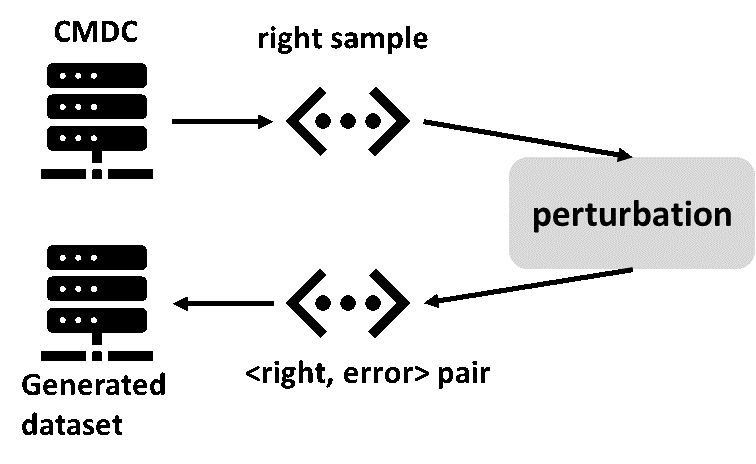
\includegraphics[width=0.8\textwidth]{AEGD.png}
    \caption{Artifical error generation for Dataset.}
    \label{fig:8}
\end{figure}

\section{Implementation}
To artificially increase the dataset amount when training the built seq2seq model, we apply the sampling strategy described above multiple times to arrive at 2-3 times of the number of input-output pairs. Given this augmented dataset, training can be executed in a similar manner to seq2seq model training of the previous existing works. That is, we train a sequence-to-sequence model using LSTM encoders and decoders with an attention mechanism as described in \cite{bahdanau2014neural} using stochastic gradient descent.

\subsection{Decoding}

Instead of using the most probable decoding according to the seq2seq model, this project takes advantage of the unique structure of this problem to impose the prior that all tokens in a decoded sequence should either exist in the input sequence or belong to a set of "corrective" tokens. The "corrective" token set is constructed during training and contains all tokens seen in the target, but not the source, for at least one sample in the training set. The intuition here is that the errors which are marked during training involve the misuse of a relatively small vocabulary of common words (e.g. "the", "an", "their") and that the model should only be allowed to perform corrections in this domain.

This prior is carried out through a modification to the seq2seq model's decoding loop in addition to a post-processing step that resolves out-of-vocabulary (OOV) tokens:

\begin{itemize}
    \item Biased Decoding: This project applies a binary mask to the model's logits prior to extracting the prediction to be fed into the next time step. This can restrict the decoding such that it only ever chooses tokens from the input sequence or corrective token set. The mask is constructed in the following way
    \begin{align}
    Mask[i]=
    \begin{cases}
        1, i \; in \; input\; or\; corrective\_tokens\\
        0, else
    \end{cases}
    \end{align}
    Since this mask is applied to the result of a softmax transformation. This transformation can guarantees all outputs are non-negative. We can be sure that only input or corrective tokens are ever selected. Note that this logic is not used during training, as this would only serve to eliminate potentially useful signal from the model.
    \item Handling OOV Tokens: Since the decoding bias described above is applied within the truncated vocabulary used by the model, we will still see the unknown token in its output for any OOV tokens. The more generic problem of resolving these OOV tokens is non-trivial (e.g. see Addressing the Rare Word Problem in NMT), but in this project we can again take advantage of its unique structure to create a straightforward OOV token resolution scheme. That is, if we assume the sequence of OOV tokens in the input is equal to the sequence of OOV tokens in the output sequence, then we can trivially assign the appropriate token to each "unknown" token encountered in the decoding. Empirically, and intuitively, this appears to be an appropriate assumption, as the relatively simple class of errors these models are being trained to address should never include mistakes that warrant the insertion or removal of a rare token.
\end{itemize}

\subsection{Details}
This project reuses and slightly extends TensorFlow's Seq2SeqModel, which itself implements a sequence-to-sequence model with an attention mechanism as described in tensorflow’s tutorial document. The primary function file we use is described as the following:
\begin{itemize}
    \item \texttt{data\_reader.py}: an abstract class that defines the interface for classes which can read a source dataset and producing input-output pairs, where the input is a grammatically incorrect variant of a source sentence and the output is the original sentence.
    \item \texttt{text\_corrector\_data\_readers.py}: contains a few implementations of DataReader which is over the CMDC.
    \item \texttt{text\_corrector\_models.py}: contains a version of Seq2SeqModel modified such that it implements the logic described in Biased Decoding.
    \item \texttt{correct\_text.py}: a collection of helper functions that together allow for the training of a model and the usage of it to decode errant input sequences (at test time). The decode method defined here implements the OOV token resolution logic. This also defines a main method and can be invoked from the command line. It was largely derived from TensorFlow's translate.py.
\end{itemize}


\chapter{Experiments and Results}
\label{chapter6}

In this section, we will describe how we do the experience and the final result of our GEC system. In the experiment part, we mainly train the seq2seq model, do test by applying sample sentence and analysis the model structure and performance.

\section{Experiment Environment}
The software and hardware environments are shown in the following table:
\begin{table}[ht]
\centering
\begin{tabular}{|c | c |} 
    \hline
    GPU & NVIDIA TITAN V $\times2$ \\  
    \hline
    Operating System & Ubuntu 16.04.6 LTS \\ 
    \hline
    Python Version & 3.5.2 (must be this version) \\
    \hline
    Libraries & tensorflow 0.12.0, nltk, pandas, scikit-learn, collections \\ 
    \hline
\end{tabular}
\caption{Environment}
\label{table:1}
\end{table}

\section{Parameters}
The dataset consists of 304,713 lines from movie scripts, of which 243,768 lines were used to train the model and 30,474 lines each were used for the validation and testing sets. The sets were selected such that no lines from the same movie were present in both the training and testing sets.
The model being evaluated below is a sequence-to-sequence model, with attention, where the encoder and decoder were both 2-layer, 512 hidden unit LSTMs. The model was trained with a vocabulary of the 2k most common words seen in the training set.
\section{Performance evaluation}
In the experiment, we run a base line and our model. Here, the baseline is the identity function, which means that we assume no errors exist in the input. To evaluate the performance of the developed GEC system, we apply BLEU score. BLEU score is an algorithm for evaluating the quality of text which has been machine-translated from one natural language to another. The closer the output sentence is to the correct on, the higher the BLEU score is.

The formulation of BLEU score is defined as below.
\begin{align}
    \text{BLEU}=\min(1, \frac{\text{output length}}{reference length})(\prod_{i=1}^{4}\text{precision}_{i})^{\frac{1}{4}}
\end{align}

We sample the sentence from the testing dataset to check the performance. The result is shown in the following.
\begin{figure}
\centering
\begin{subfigure}{.5\textwidth}
    \centering
    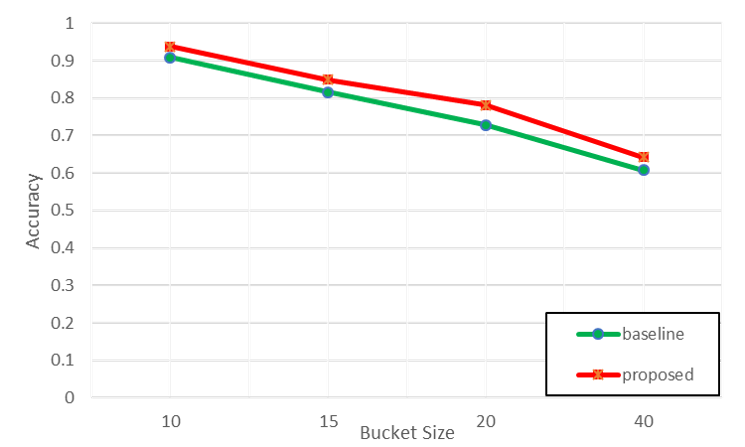
\includegraphics[width=.9\linewidth]{ACCU1.png}
    \caption{Accuracy vs. Bucket Size}
    \label{fig:sub1}
\end{subfigure}%
\begin{subfigure}{.5\textwidth}
    \centering
    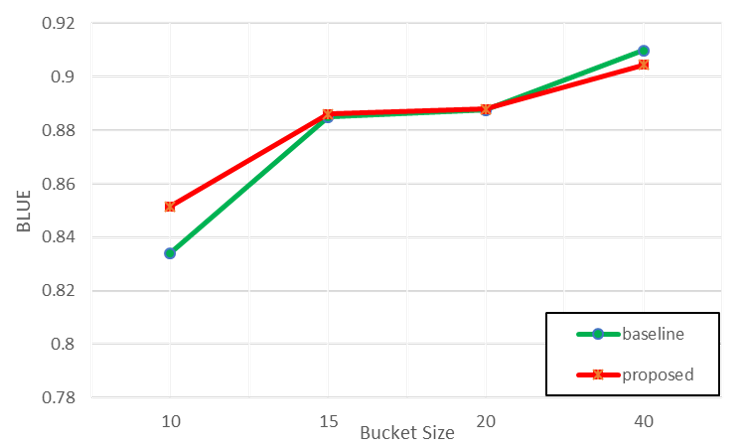
\includegraphics[width=.9\linewidth]{BLUE1.png}
    \caption{BLUE score vs. Bucket Size}
    \label{fig:sub2}
\end{subfigure}
\caption{Results of proposed model and baseline for different bucket size after 40000 times when coveraging.}
\label{fig:9}
\end{figure}
From Figure~\ref{fig:9}, we can notice that the trained GEC system outperforms this baseline for all bucket sizes in terms of accuracy. The GEC system also outperforms the baseline except only case in terms of BLEU score. This tells us that applying the seq2seq model with LSTM to a potentially errant writing sample would, on average, results in a more grammatically correct writing sample. 

In addition, how the performance of the trained model change with the number of iteration. If the performance of the trained model become worse at the large number region, we may need to do ``early stop'' trick for the training.
\begin{figure*}
    \centering
    \begin{subfigure}[b]{0.475\textwidth}
        \centering
        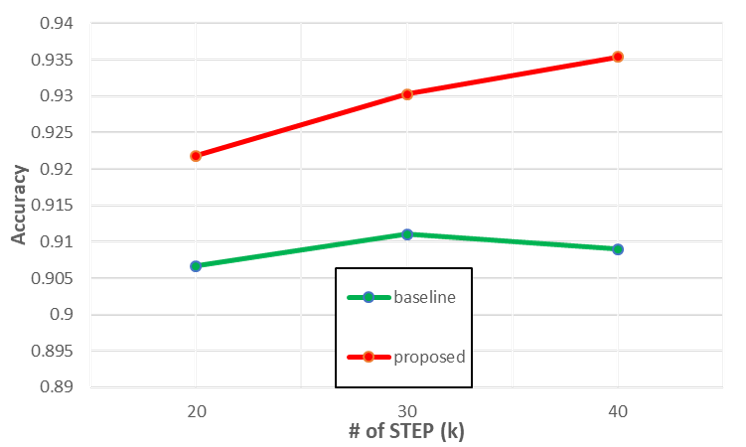
\includegraphics[width=\textwidth]{ACCU10.png}
        \caption[]%
        {{\small Accuracy vs. step number for Bucket size $= 10$}}    
        \label{fig:ACCU10}
    \end{subfigure}
    \hfill
    \begin{subfigure}[b]{0.475\textwidth}  
        \centering 
        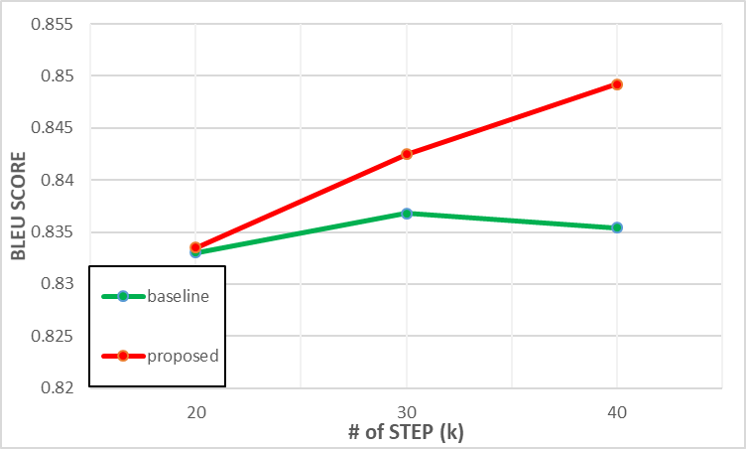
\includegraphics[width=\textwidth]{BLUE10.png}
        \caption[]%
        {{\small BlEU Score vs. step number for Bucket size $= 10$}}    
        \label{fig:BLUE10}
    \end{subfigure}
    \vskip\baselineskip
    \begin{subfigure}[b]{0.475\textwidth}
        \centering
        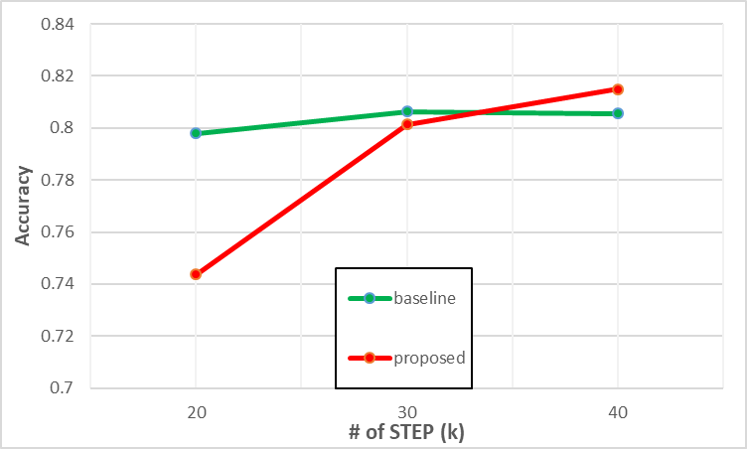
\includegraphics[width=\textwidth]{ACCU15.png}
        \caption[]%
        {{\small Accuracy vs. step number for Bucket size $= 15$}}    
        \label{fig:ACCU15}
    \end{subfigure}
    \hfill
    \begin{subfigure}[b]{0.475\textwidth}  
        \centering 
        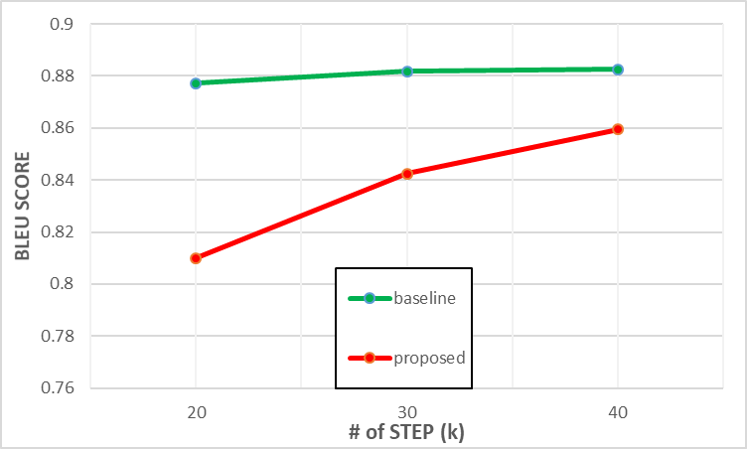
\includegraphics[width=\textwidth]{BLUE15.png}
        \caption[]%
        {{\small BlEU Score vs. step number for Bucket size $= 15$}}    
        \label{fig:BLUE15}
    \end{subfigure}
    \vskip\baselineskip
    \begin{subfigure}[b]{0.475\textwidth}
        \centering
        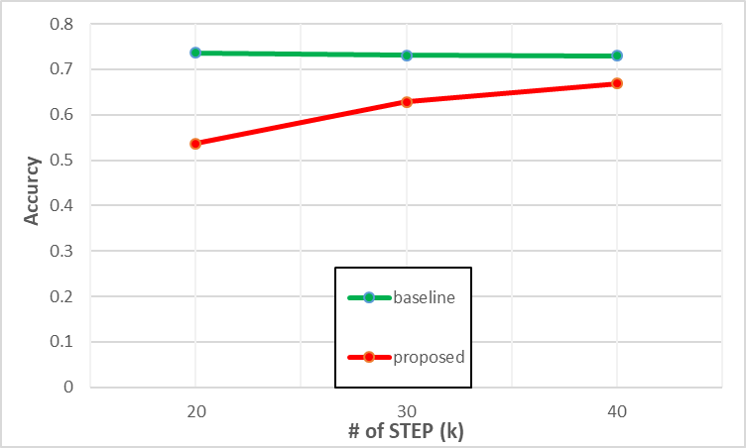
\includegraphics[width=\textwidth]{ACCU20.png}
        \caption[]%
        {{\small Accuracy vs. step number for Bucket size $= 20$}}    
        \label{fig:ACCU20}
    \end{subfigure}
    \hfill
    \begin{subfigure}[b]{0.475\textwidth}  
        \centering 
        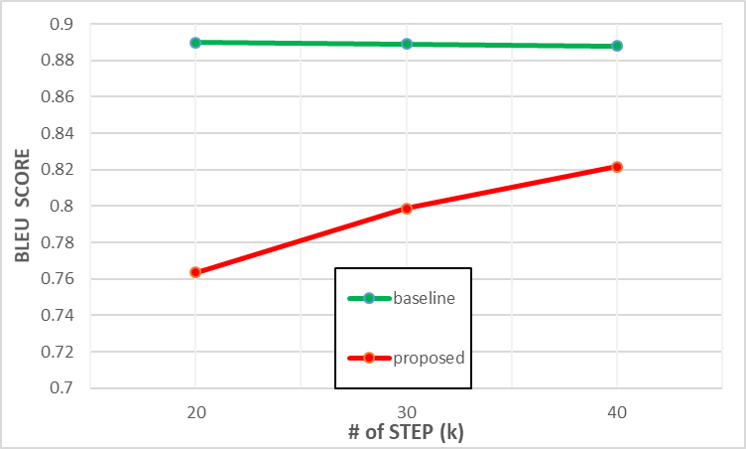
\includegraphics[width=\textwidth]{BLUE20.png}
        \caption[]%
        {{\small BlEU Score vs. step number for Bucket size $= 20$}}    
        \label{fig:BLUE20}
    \end{subfigure}
    \vskip\baselineskip
    \begin{subfigure}[b]{0.475\textwidth}   
        \centering 
        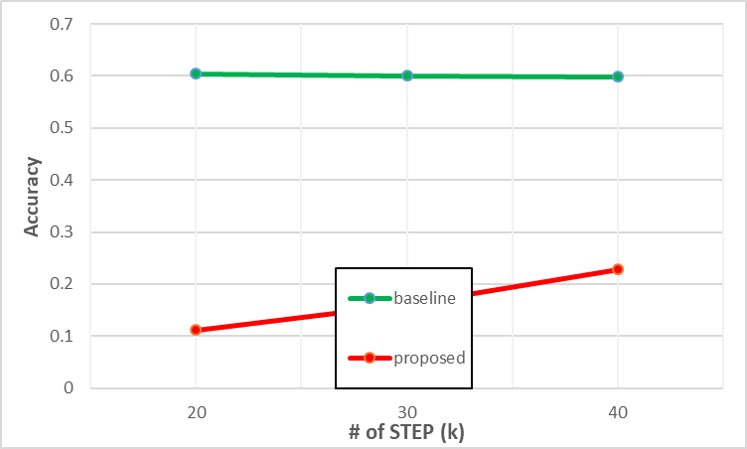
\includegraphics[width=\textwidth]{ACCU40.png}
        \caption[]%
        {{\small Accuracy vs. step number for Bucket size $= 40$}}    
        \label{fig:ACCU40}
    \end{subfigure}
    \quad
    \begin{subfigure}[b]{0.475\textwidth}   
        \centering 
        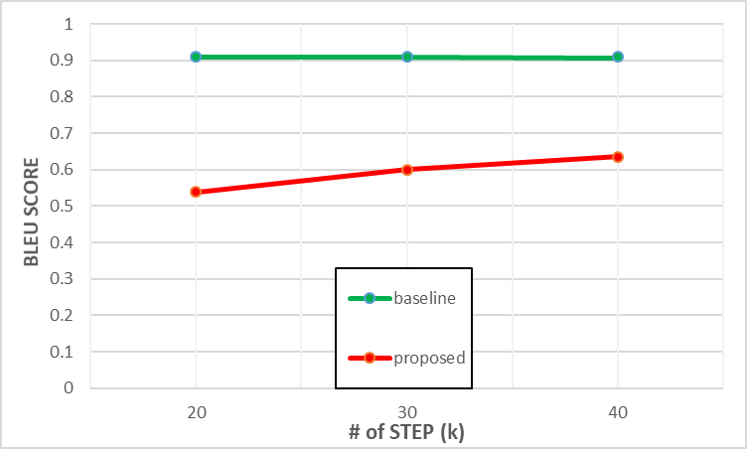
\includegraphics[width=\textwidth]{BLUE40.png}
        \caption[]%
        {{\small BlEU Score vs. step number for Bucket size $= 40$}}    
        \label{fig:BLUE40}
    \end{subfigure}
    \caption[]
    {\small Performance vs. step number for different Bucket size} 
    \label{fig:performance}
\end{figure*}
The results are shown in Figure~\ref{fig:performance}.
From Figure~\ref{fig:performance}, we can get the following conclusions.
\begin{itemize}
    \item The performance of the trained models are better for the smaller bucket size. From Figure~\ref{fig:performance} and Figure~\ref{fig:9}, we can see that the trained model of bucket size $=10$ can outperforms the baseline for different iteration step numbers. For the hyper-parameter bucket size, it is recommended to set bucket size to smaller value instead a larger one.
    \item As the number of iteration step increases, the performance of the trained model become better. It means that the model does not show overfit within 40000 steps.
    \item The trained model is not always better than the baseline. From Figure~\ref{fig:performance}, the performance of the trained model is worse than the baseline in six subfigures. Thus, the hyper-parameters should be carefully tuned.
\end{itemize}

\section{Examples}
The following Figure shows some case we test for the GEC system. This shows that the GEC system can Decoding a sentence with a missing article. From the figure, we can also see that there are still many typos the GEC system cannot detect. However, overall, the performance of the trained GEC system is acceptable.
\begin{figure}[ht]
    \centering
    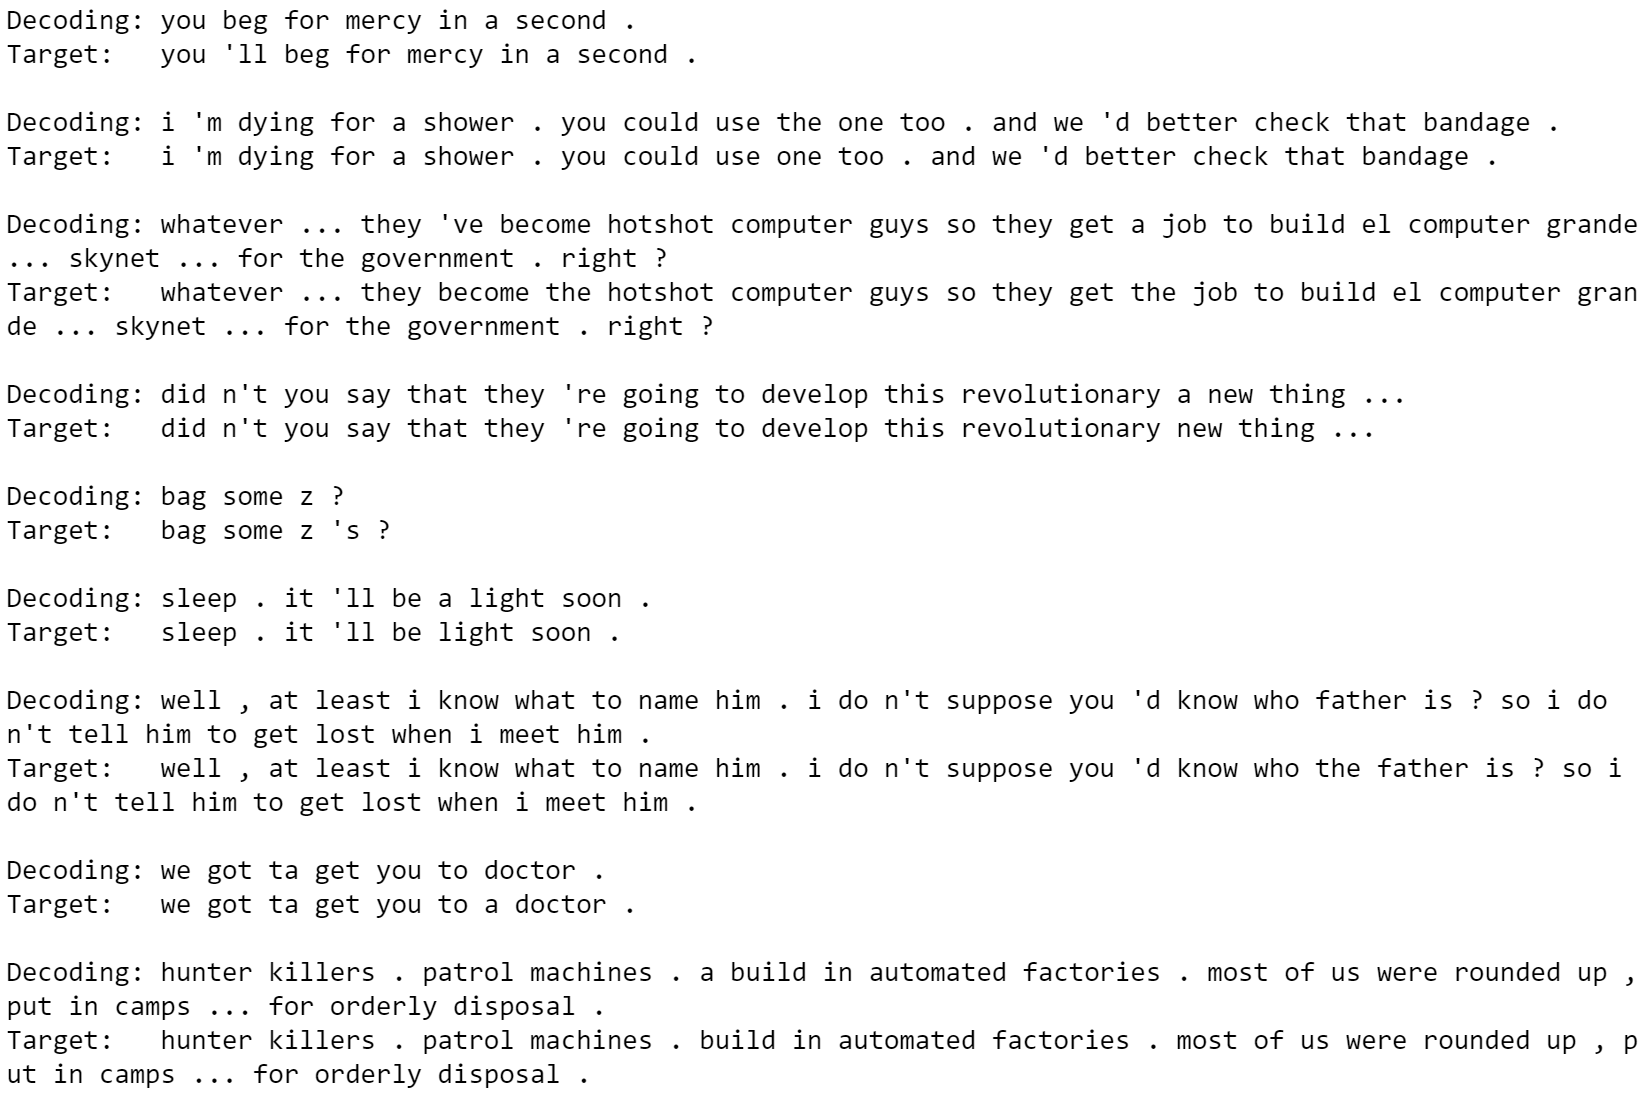
\includegraphics[width=0.8\textwidth]{testcase.png}
    \caption{Test Cases.}
    \label{fig:10}
\end{figure}
\chapter{Conclusions}
\label{chapter7}

In conclusion, this paper has a review of the exist techniques of automatic grammatical error correction system. This project developed an automatic system which can detect and correct the grammatical errors automatically. Instead of the traditional statistic model and manually rule design, we use TensorFlow to build up a seq2seq model with LSTM and train the model on a GPU server and do performance test of it. Besides, we also overcome the lack of training dataset, i.e., we take English text samples which are known to be mostly grammatically correct and randomly introducing a handful of small grammatical errors to each sentence to produce input-output. The trained GEC system outperforms this baseline for all bucket sizes in terms of both accuracy and BELU score. 
\chapter{Future Works}
\label{chapter8}

Although the developed GEC system can detect and correct some typical grammatical error happens in writing, it cannot detect the types which do not appear the training dataset. The GEC system still be further improved in the following aspects.
\begin{itemize}
    \item Add more error types into the training dataset. So far, there are only three types of grammatical errors. Diverse error type in dataset can improve the detection ability of the GEC system.
    \item The architecture of GEC system can be further improved. Maybe, a multilayer convolutional encoder-decoder neural network can be adopted into the GEC system.
\end{itemize}

%Adds References to the table of content
%all you bibtex enteries go in the file called refs.bib
\addcontentsline{toc}{chapter}{References}
\bibliography{refs}

%any appendices you have go in a file called appendix.
\begin{appendices}
\chapter{Instruction to execution}
\section{File Structure}
The environment must be installed as the Table~\ref{table:1}. 
It is recommended to use anaconda and set up a virtual environment. GPU server is recommended to use. It will take about 24 hours to train by NVIDIA TITAN V $\times2$.
The file structure is shown as following:
\begin{figure}[ht]
    \centering
    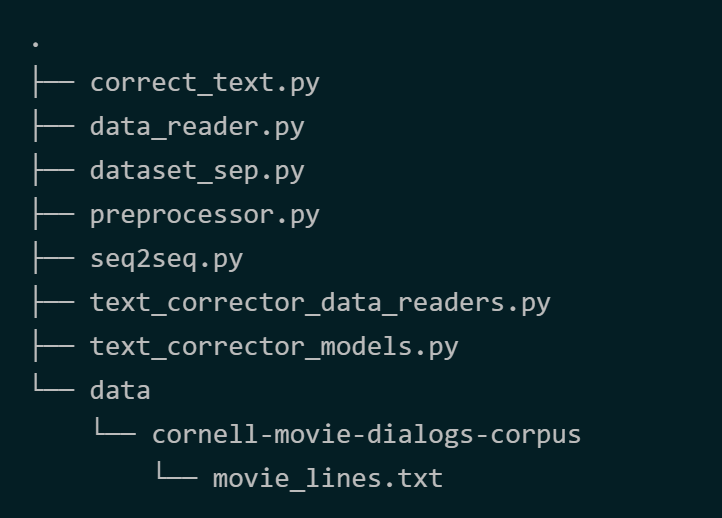
\includegraphics[width=0.8\textwidth]{filest.png}
    \caption{File Structure.}
    \label{fig:11}
\end{figure}
\section{Train and Test}
The following command can be used for training.
\begin{lstlisting}
correct_text.py     --train_path PATH OF TRAINING DATA
                    --val_path PATH OF VALIDATING DATA
                    --config DefaultMovieDialogConfig 
                    --data_reader_type MovieDialogReader
                    --model_path PATH OF SAVED MODEL
\end{lstlisting}
After training, the trained model can be loaded by the following command.
\begin{lstlisting}
model = create_model(sess, True, model_path, config=config)
\end{lstlisting}
To test the trained model, the following command can used.
\begin{lstlisting}
correct_text.py     --test_path PATH OF TESTING DATA
                    --config DefaultMovieDialogConfig 
                    --data_reader_type MovieDialogReader 
                    --model_path /movie_dialog_model
                    --decode
\end{lstlisting}

\end{appendices}
\end{document}

